Постановка авторегрессионнного моделирования, включающая предсказание следующего слова по предшествующему контексту,
может быть использована для решения ключевых для обработки языка задач перевода, пересказа и выделения ключевых слов. 
Дная техника позволила исследователям \cite{radford2021learning} обучить
общую модель работы с текстом GPT (генеративный обучающий трансформер). Отличительной особенностью исследования была его
масштабность. Модель обучена на объеме более триллиона слова, полученного с помощью выделения естественного языка из источников в internet.
Таким образом, в краткие сроки были приобретены навыки распознания и генерации на более чем ста языках мира и базовые знания об естественных и социальных науках.
Для прохождения испытаний по метрической оценке навыков модели были использованы корпуса высокого качества. 

\begin{figure}[h]
    \centering
    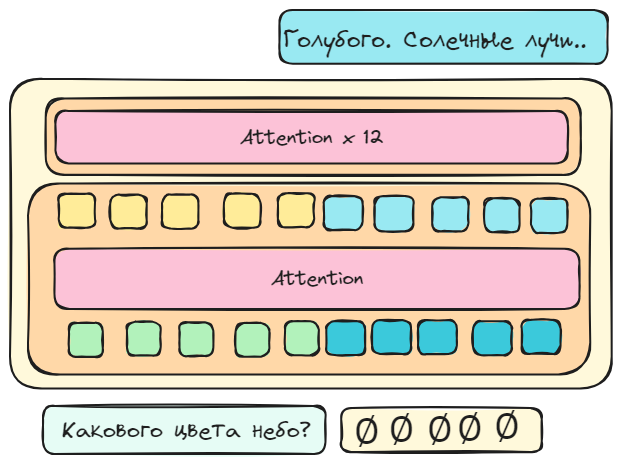
\includegraphics[width=0.5\textwidth]{assets/ml/nlp/gpt.excalidraw.png}
    \caption{Большая языковая модель GPT обучается как авторегрессионная модель на задаче предсказания следующего слова}
    \label{gpt}
\end{figure}

Обучение языковых моделей для задач ассистирования разделяется на три этапа \cite{ouyang2022training}: \begin{enumerate}
    \item предобучение, включающее формирование представлений о синтаксической структуре языков мира, модели мира и 
    разнообразии формы выражения мысли;
    \item адаптацию под задачу, знакомящую модель с терминами и связями между ними;
    \item инструкционное дообучение, заключающееся в обучение модели выполнять задачи, необходимые в практике специалистов.
\end{enumerate}
В ходе первого этапа модель обучается на обширных разнородных корпусах текста. Предобучение требует значительных 
вычислительных ресурсов, не всегда доступных в образовательных и научных приложениях, поэтому в исследованиях используются
открытые языковые модели, опубликованные коммерческими организациями \cite{jiang2023mistral} \cite{jiang2024mixtral} \cite{touvron2023llama}.
Второй этап обучения выполняется на экспертно отобранном корпусе предметных документов. В сфере образования таковыми являются цифровая учебная
литература, вопросы и ответы на предметных форумах и научные статьи. Данные для эффективного обучения должны 
иметь максимально возможное качество: необходимо исправлять ошибки набора и неструктурированные в соответствии с правилами
языка фрагменты текста. В противном случае, модель может запомнить неверные правила форматирования \cite{zhao2023survey}.
Финальный этап начинается с обучения на стандартном корпусе инструкций, включающих базовые задачи  структурированных определений, изложение информации в требуемой
стилистической форме и поиск ключевых слов \cite{zhang2023instruction}. На данном этапе модель уже способна эвристически решать 
большое число задач, но может ошибаться в специфических постановках. Для их устранения этих недостатков 
эксперты корректируют ошибочные решения модели. Таким образом модель одновременно приобретает навыки правильного решения
и получает информацию о видах нежелательных ответов. 

\begin{figure}[h]
    \centering
    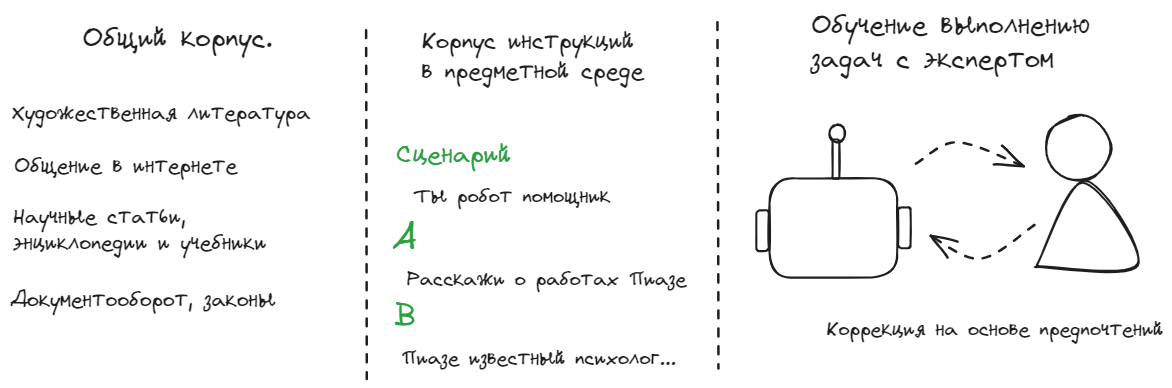
\includegraphics[width=0.75\textwidth]{assets/work/arch/learning.excalidraw.png}
    \caption{Обучение разбито на три ключевых этапа: подготовка, адаптация на корпусе и экспертная коррекция}
    \label{train}
\end{figure}

Для оценки способностей языковых моделей создаются специальные системы тестирования, количественно оценивающие способности моделей к:
\begin{itemize}
    \item владение языками мира \cite{hendrycks2020measuring};
    \item способности к эффективному ведению диалога \cite{zhong2023agieval};
    \item пониманию животного и растительного мира, социальных правил и законов \cite{chollet2019measure} \cite{guha2024legalbench};
    \item решения аналитических и абстрактных логических задач \cite{rein2023gpqa} \cite{cobbe2021training}.
\end{itemize}

\begin{figure}[h]
    \centering
    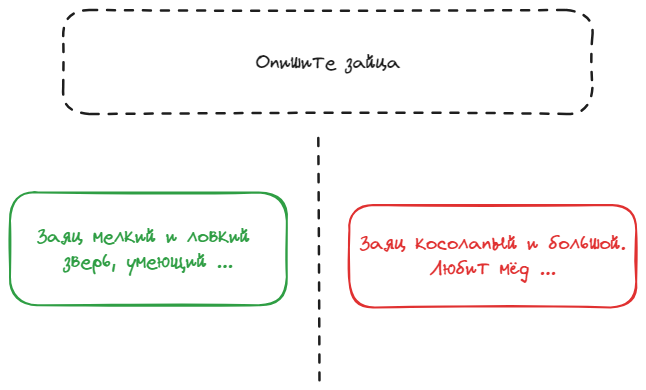
\includegraphics[width=0.5\textwidth]{assets/work/arch/instruction.excalidraw.png}
    \caption{Адаптация к задачам выполняется путем взаимодействия с пользователем и работой с экспертом}
    \label{instruction}
\end{figure}


Отметим, что современные большие языковые модели не гарантируют корректное исполнение даже базовых арифметических операций. В обзоре \cite{zhao2023survey} показано, 
что подобные проблемы возникают во многих строгих постановках, где соблюдение формы требует 
более глубокого чем эвристического понимания задачи:
\begin{itemize}
    \item написание исполняемого языком программирования кода;
    \item стратегические игры \cite{Adam2024};
    \item соблюдение корректности математических выражений при алгебраических преобразованиях.
\end{itemize} 

Для решения проблемы исследователи предложили использование инструментов, которые используются моделью для качественного
выполнения инструкции. На данный момент сложились следующие подходы:
\begin{itemize}
    \item обращения к информационным системам (от \textit{англ.} RAG - retrieval augmented generation)\cite{lewis2020retrieval};
    \item работа с средой исполнения программного кода \cite{parisi2022talm};
    \item генерация сопровождающей иллюстрации \cite{rombach2022high}.
\end{itemize}










